% =====================================================================
% Beamer slide deck for Chapter 11 "Cloud Security"
%
% Source of content: chapters/chapter11_cloud_security.tex
%   (Manvi & Shyam, "Cloud Computing: Concepts and Technologies",
%    CRC Press, 2021, Chapter 11, pp. 205-227)
%
% Slides are in English; terminology follows the English terms carried
% in the chapter file. The chapter file itself is NOT modified.
%
% Build (from the project root):
%   xelatex -output-directory=slides slides/chapter11.tex
% or (from this directory):
%   xelatex chapter11.tex
% =====================================================================
\documentclass[11pt,aspectratio=169]{beamer}

\usepackage{fontspec}
\setsansfont{Liberation Sans}
\usefonttheme{professionalfonts}

\usepackage{amsmath,amssymb}
\usepackage{graphicx}
\usepackage{booktabs}
\usepackage{tikz}
\usetikzlibrary{arrows.meta,positioning,shapes.geometric,calc,fit,backgrounds}

% Works whether compiled from the project root or from slides/
\graphicspath{{assets/images/}{../assets/images/}}

% ---------------------------------------------------------------------
% A minimal, clean academic theme. The project had no existing Beamer
% convention, so this file defines one: a single accent colour, no
% navigation clutter, a thin title rule and a plain footline.
% ---------------------------------------------------------------------
\usetheme{default}
\setbeamertemplate{navigation symbols}{}

\definecolor{accent}{HTML}{1F4E79}
\definecolor{accentmid}{HTML}{2E75B6}
\definecolor{accentsoft}{HTML}{EAF1F8}
\definecolor{inkgrey}{HTML}{444444}
\definecolor{warmred}{HTML}{A33A30}

\setbeamercolor{normal text}{fg=inkgrey}
\setbeamercolor{structure}{fg=accent}
\setbeamercolor{alerted text}{fg=warmred}
\setbeamercolor{title}{fg=accent}
\setbeamercolor{subtitle}{fg=accentmid}
\setbeamercolor{frametitle}{fg=accent}
\setbeamercolor{block title}{fg=white,bg=accent}
\setbeamercolor{block body}{bg=accentsoft}
\setbeamercolor{itemize item}{fg=accentmid}
\setbeamercolor{itemize subitem}{fg=accentmid}
\setbeamercolor{section in toc}{fg=accent}

\setbeamertemplate{itemize item}{\raisebox{0.12ex}{\tiny$\blacksquare$}}
\setbeamertemplate{itemize subitem}{\raisebox{0.12ex}{\tiny$\square$}}
\setbeamerfont{frametitle}{size=\large,series=\bfseries}
\setbeamerfont{title}{size=\LARGE,series=\bfseries}
\setbeamerfont{block title}{size=\small,series=\bfseries}

% Frame title: bold text over a thin accent rule.
\setbeamertemplate{frametitle}{%
  \vspace{1.2ex}%
  \begin{beamercolorbox}[wd=\paperwidth,leftskip=0.9cm,rightskip=0.9cm]{frametitle}%
    \usebeamerfont{frametitle}\insertframetitle\par
    \vspace{0.6ex}%
    {\color{accentmid}\rule{\dimexpr\paperwidth-1.8cm\relax}{0.7pt}}%
  \end{beamercolorbox}%
}

% Footline: short title on the left, frame number on the right.
\setbeamertemplate{footline}{%
  \hbox{\begin{beamercolorbox}[wd=\paperwidth,ht=2.6ex,dp=1.4ex,
        leftskip=0.9cm,rightskip=0.9cm]{}%
    {\scriptsize\color{accentmid}Chapter 11 \textbar{} Cloud Security}%
    \hfill
    {\scriptsize\color{accentmid}\insertframenumber}%
  \end{beamercolorbox}}%
}

\newcommand{\kw}[1]{\textbf{\color{accent}#1}}

% Shared TikZ styles
\tikzset{
  boxy/.style   = {rounded corners=2pt, draw=accentmid, fill=accentsoft,
                   text=inkgrey, align=center, inner sep=5pt, font=\scriptsize},
  solidbox/.style = {rounded corners=2pt, draw=accent, fill=accent,
                   text=white, align=center, inner sep=5pt, font=\scriptsize\bfseries},
  redbox/.style = {rounded corners=2pt, draw=warmred, fill=warmred!8,
                   text=inkgrey, align=center, inner sep=5pt, font=\scriptsize},
  flow/.style   = {-{Stealth[length=2mm]}, draw=accentmid, thick},
  flowred/.style= {-{Stealth[length=2mm]}, draw=warmred, thick},
}

% ---------------------------------------------------------------------
\title{Cloud Security}
\subtitle{Chapter 11 \textbar{} Cloud Computing: Concepts and Technologies}
\author{Sunilkumar S. Manvi \and Gopal Krishna Shyam}
\institute{CRC Press, 2021}
\date{}

\begin{document}

% ===================== 1. Title =====================
\begin{frame}[plain]
  \titlepage
  \vfill
  {\footnotesize\color{accentmid}Slides derived from Chapter 11, pp. 205--227.}
\end{frame}

% ===================== 2. Outline =====================
\begin{frame}{Outline}
  \vspace{0.5em}
  \begin{columns}[T,onlytextwidth]
    \begin{column}{0.5\textwidth}
      \begin{enumerate}\setlength{\itemsep}{0.7em}\small
        \item[\textbf{11.1}] Data Security
        \item[\textbf{11.2}] Encryption Techniques in Cloud
        \item[\textbf{11.3}] Infrastructure Security
        \item[\textbf{11.4}] PaaS Application Security
      \end{enumerate}
    \end{column}
    \begin{column}{0.5\textwidth}
      \begin{enumerate}\setlength{\itemsep}{0.7em}\small
        \item[\textbf{11.5}] SaaS Application Security
        \item[\textbf{11.6}] Securing Virtual Servers
        \item[\textbf{11.7}] Cloud Security Controls
      \end{enumerate}
    \end{column}
  \end{columns}
  \vspace{1.2em}
  \begin{block}{Learning objectives}
    \small
    Assess data security in the Cloud \textbullet{} describe security management
    in the Cloud \textbullet{} compare and contrast IaaS, PaaS and SaaS security
    in Cloud deployments.
  \end{block}
\end{frame}

% ===================== 3. What cloud security is =====================
\begin{frame}{What Cloud Security Covers}
  \begin{columns}[T,onlytextwidth]
    \begin{column}{0.54\textwidth}
      \small
      A sub-domain of \kw{computer security}, \kw{network security} and,
      more broadly, \kw{data security}.
      \vspace{0.8em}

      Applies across all\dots
      \begin{itemize}\small
        \item \textbf{Service models:} SaaS, PaaS, IaaS
        \item \textbf{Deployment models:} private, hybrid, public, community
      \end{itemize}
      \vspace{0.8em}

      Security concerns split into two categories: those faced by
      \kw{providers} and those faced by \kw{clients}.
    \end{column}
    \begin{column}{0.44\textwidth}
      \centering
      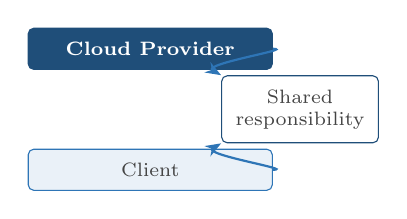
\begin{tikzpicture}[node distance=6mm]
        \node[solidbox,minimum width=3.1cm] (p) {Cloud Provider};
        \node[boxy,below=10mm of p,minimum width=3.1cm] (c) {Client};
        \node[boxy,right=9mm of $(p)!0.5!(c)$,minimum width=1.9cm,
              fill=white,draw=accent] (s) {Shared\\responsibility};
        \draw[flow] (p.east) to[out=0,in=150] (s.north west);
        \draw[flow] (c.east) to[out=0,in=210] (s.south west);
      \end{tikzpicture}

      \vspace{0.8em}
      {\scriptsize
      \textbf{Provider:} services are secure; customer data and
      applications are protected.\par
      \vspace{0.4em}
      \textbf{Client:} supports those measures, e.g.\ strong passwords.}
    \end{column}
  \end{columns}
\end{frame}

% ===================== 4. CIA triad =====================
\begin{frame}{Preliminaries: Confidentiality, Integrity, Availability}
  \begin{columns}[T,onlytextwidth]
    \begin{column}{0.42\textwidth}
      \centering
      \vspace{0.5em}
      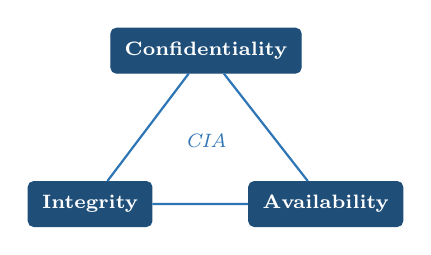
\begin{tikzpicture}[scale=0.95]
        \node[solidbox] (c) at (0,2.05) {Confidentiality};
        \node[solidbox] (i) at (-1.55,0) {Integrity};
        \node[solidbox] (a) at (1.6,0) {Availability};
        \draw[accentmid,thick] (c) -- (i) -- (a) -- (c);
        \node[font=\scriptsize\itshape,color=accentmid] at (0,0.85) {CIA};
      \end{tikzpicture}
    \end{column}
    \begin{column}{0.56\textwidth}
      \small
      \begin{itemize}\setlength{\itemsep}{0.7em}
        \item \kw{Confidentiality:} prevention of intentional or unintentional
              unauthorized disclosure of contents.
        \item \kw{Integrity:} assurance that the message sent is the message
              received, and was not changed on the way.
        \item \kw{Availability:} the components that create reliability and
              stability, so authorized clients reach the system when needed.
      \end{itemize}
    \end{column}
  \end{columns}
  \vspace{0.3em}
  \begin{block}{Why it changes in the Cloud}
    \footnotesize
    A large part of network, system, applications and information moves under
    third-party control, creating islands of \kw{virtual perimeters} plus a
    security model shared between the client and the \kw{CSP}.
  \end{block}
\end{frame}

% ===================== 5. Data in transit =====================
\begin{frame}{11.1 Data Security: Data-in-Transit}
  \small
  Data-in-transit identifies \kw{data that requires encryption} while moving
  from one device to another.
  \vspace{0.9em}

  \begin{columns}[T,onlytextwidth]
    \begin{column}{0.32\textwidth}
      \begin{block}{Public networks}
        \scriptsize
        Transfer over the Internet, e.g.\ a mobile app calling a banking
        service. Typically encrypted using protocols such as HTTP.
      \end{block}
    \end{column}
    \begin{column}{0.32\textwidth}
      \begin{block}{Private networks}
        \scriptsize
        Transfer over a secured LAN. \emph{Defense in depth:} do not trust that
        a network is properly secured. Apply the same encryption as on public
        networks.
      \end{block}
    \end{column}
    \begin{column}{0.32\textwidth}
      \begin{block}{Local devices}
        \scriptsize
        Transfer between computers, storage devices and peripherals. The medium
        itself can intercept, e.g.\ a USB cord that records or transmits.
      \end{block}
    \end{column}
  \end{columns}
\end{frame}

% ===================== 6. Categories, risk, metadata =====================
\begin{frame}{11.1 Data-in-Transit: Categories and Primary Risk}
  \small
  \textbf{Two categories}
  \begin{enumerate}\small\setlength{\itemsep}{0.3em}
    \item Information flowing over a \kw{public or untrusted} network, such as
          the Internet.
    \item Data flowing within the confines of a \kw{private} network, such as a
          corporate or enterprise LAN.
  \end{enumerate}
  \vspace{0.8em}

  \begin{alertblock}{Primary risk}
    \small
    Not using a \kw{vetted encryption algorithm}. Obvious to security
    professionals, but often not understood by others using a public Cloud,
    whether IaaS, PaaS or SaaS.
  \end{alertblock}
  \vspace{0.4em}

  \begin{block}{Beyond the data itself: metadata}
    \small
    What metadata does the provider hold about the data, how is it secured, and
    what access does the customer have to it? As data volume with a provider
    grows, \kw{so does the value of that metadata}.
  \end{block}
\end{frame}

% ===================== 7. Security concerns =====================
\begin{frame}{11.1 Significant Security Concerns in the Cloud}
  \small
  Cloud computing spans networks, databases, operating systems,
  virtualization, resource scheduling, transaction management, load balancing,
  concurrency control and memory management.
  \vspace{0.8em}

  \begin{columns}[T,onlytextwidth]
    \begin{column}{0.49\textwidth}
      \begin{itemize}\small\setlength{\itemsep}{0.45em}
        \item \kw{Data transmission} over a communication medium
        \item \kw{Virtualization security} of the virtual environment
        \item \kw{Network security} of assets and traffic
        \item \kw{Data integrity}: what may be shared with third parties
      \end{itemize}
    \end{column}
    \begin{column}{0.49\textwidth}
      \begin{itemize}\small\setlength{\itemsep}{0.45em}
        \item \kw{Data privacy}: accuracy and consistency of stored data
        \item \kw{Data location}: logical pools across many servers
        \item \kw{Data availability}: from normal through ``disastrous''
              situations
      \end{itemize}
    \end{column}
  \end{columns}
  \vspace{0.7em}
  {\footnotesize\color{accentmid}
  Two examples of what must be secured: the network interconnecting systems in
  a Cloud, and the mapping of virtual machines onto physical machines.}
\end{frame}

% ===================== 8. Encryption overview =====================
\begin{frame}{11.2 Encryption Techniques in Cloud}
  \small
  \kw{Cloud encryption} transforms a Cloud service customer's data into
  \kw{ciphertext} before it is placed on a storage Cloud.
  \vspace{0.9em}

  \begin{columns}[T,onlytextwidth]
    \begin{column}{0.32\textwidth}
      \begin{block}{ABE}
        \scriptsize
        \textbf{Attribute-based encryption.} Public-key encryption where the
        secret key and the ciphertext depend on \emph{attributes}. Decryption
        works only if the attribute sets match.
      \end{block}
    \end{column}
    \begin{column}{0.32\textwidth}
      \begin{block}{FHE}
        \scriptsize
        \textbf{Fully homomorphic encryption.} Allows computation on encrypted
        data, including sum and product, \emph{without decryption}.
      \end{block}
    \end{column}
    \begin{column}{0.32\textwidth}
      \begin{block}{SE}
        \scriptsize
        \textbf{Searchable encryption.} Secure search over encrypted data.
        Split into secret-key (symmetric) and public-key SE.
      \end{block}
    \end{column}
  \end{columns}
  \vspace{0.9em}
  {\footnotesize\color{accentmid}
  To improve search efficiency, symmetric-key SE generally builds
  \emph{keyword indexes} to answer user queries.}
\end{frame}

% ===================== 9. ABE variants =====================
\begin{frame}{11.2 Attribute-Based Encryption: Two Policies}
  \vspace{0.3em}
  \begin{columns}[T,onlytextwidth]
    \begin{column}{0.49\textwidth}
      \begin{block}{CP-ABE \textbar{} Ciphertext-policy}
        \small
        The \kw{encryptor} controls the access strategy.
        \vspace{0.4em}

        Main idea: focused on the design of the \kw{access structure}.
      \end{block}
    \end{column}
    \begin{column}{0.49\textwidth}
      \begin{block}{KP-ABE \textbar{} Key-policy}
        \small
        \kw{Attribute sets} describe the encrypted texts.
        \vspace{0.4em}

        \kw{Private keys} are associated with the specified policy that users
        will have.
      \end{block}
    \end{column}
  \end{columns}
  \vspace{1.1em}

  \begin{center}
  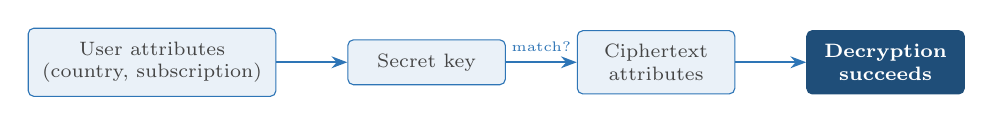
\begin{tikzpicture}[node distance=8mm]
    \node[boxy,minimum width=2.2cm] (att) {User attributes\\(country, subscription)};
    \node[boxy,right=9mm of att,minimum width=2.0cm] (key) {Secret key};
    \node[boxy,right=9mm of key,minimum width=2.0cm] (ct) {Ciphertext\\attributes};
    \node[solidbox,right=9mm of ct,minimum width=2.0cm] (dec) {Decryption\\succeeds};
    \draw[flow] (att) -- (key);
    \draw[flow] (key) -- (ct) node[midway,above,font=\tiny,color=accentmid]{match?};
    \draw[flow] (ct) -- (dec);
  \end{tikzpicture}
  \end{center}
\end{frame}

% ===================== 10. Decentralized KP-ABE =====================
\begin{frame}{11.2.1 Decentralized KP-ABE: Five Sub-modules}
  \small
  In a \kw{decentralized} scheme there is no fixed number of attribute
  authorities. Any authority can join or leave \kw{without rebooting the
  system}.
  \vspace{0.9em}

  \begin{center}
  
\begin{tikzpicture}[node distance=4.5mm]
    \node[solidbox,minimum width=2.05cm,minimum height=0.95cm] (g) {Global\\setup};
    \node[solidbox,right=of g,minimum width=2.05cm,minimum height=0.95cm] (a) {Authority\\setup};
    \node[solidbox,right=of a,minimum width=2.05cm,minimum height=0.95cm] (k) {Key\\issuing};
    \node[solidbox,right=of k,minimum width=2.05cm,minimum height=0.95cm] (e) {Encryption};
    \node[solidbox,right=of e,minimum width=2.05cm,minimum height=0.95cm] (d) {Decryption};
    \draw[flow] (g) -- (a); \draw[flow] (a) -- (k);
    \draw[flow] (k) -- (e); \draw[flow] (e) -- (d);
  \end{tikzpicture}
  \end{center}
  \vspace{0.7em}

  \begin{itemize}\scriptsize\setlength{\itemsep}{0.32em}
    \item \kw{Global setup:} security parameter in, system parameters out, for
          any authority that joins.
    \item \kw{Authority setup:} each authority generates public and private
          keys for the attributes it maintains.
    \item \kw{Key issuing:} user and authority interact through an
          \emph{anonymous key issuing protocol}; the authority returns
          decryption credentials.
    \item \kw{Encryption:} takes an attribute set plus the data, outputs the
          ciphertext.
    \item \kw{Decryption:} succeeds \emph{if and only if} the user attributes
          satisfy the access structure.
  \end{itemize}
\end{frame}

% ===================== 11. Security game =====================
\begin{frame}{11.2.2 Security Game: The Selective ID Model}
  \small
  ABE schemes are proven secure against the \kw{selective identity (ID) model},
  represented as a game between an \kw{adversary} and a \kw{challenger}.
  \vspace{0.7em}

  \begin{columns}[T,onlytextwidth]
    \begin{column}{0.52\textwidth}
      \begin{enumerate}\scriptsize\setlength{\itemsep}{0.35em}
        \item \textbf{Secret key queries.} Any number of queries, but each user
              must have at least one \emph{non-corrupted} authority.
        \item \textbf{Challenge.} Adversary sends $m_0$ and $m_1$ in plain
              domain; challenger encrypts one at random.
        \item \textbf{More secret key queries,} subject to the same
              requirement.
        \item \textbf{Guess.} Adversary names the encrypted message.
      \end{enumerate}
    \end{column}
    \begin{column}{0.46\textwidth}
      \begin{block}{Success condition}
        \small
        The adversary succeeds if it guesses correctly with probability
        \[ \frac{1}{2} + \epsilon \]
        where $\epsilon$ is a \kw{non-negligible function}.
      \end{block}
      \vspace{0.3em}
      {\scriptsize\color{accentmid}
      If the adversary cannot decrypt with non-negligible advantage, the scheme
      is secure against the selective ID model.}
    \end{column}
  \end{columns}
\end{frame}

% ===================== 12. FHE architecture =====================
\begin{frame}{11.2.3 Fully Homomorphic Encryption: Participants}
  \small
  Multiple parties play three key roles in the secure computation.
  \vspace{0.6em}

  \begin{center}
  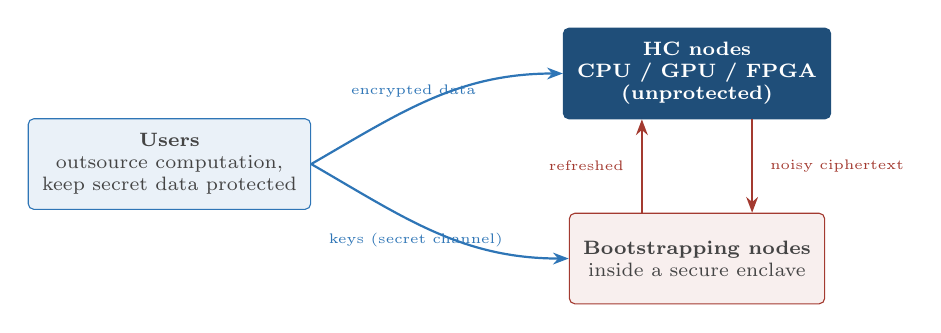
\begin{tikzpicture}
    \node[boxy,minimum width=2.9cm,minimum height=1.15cm] (u) at (0,0)
      {\textbf{Users}\\outsource computation,\\keep secret data protected};
    \node[solidbox,minimum width=2.9cm,minimum height=1.15cm] (hc) at (6.7,1.15)
      {\textbf{HC nodes}\\CPU / GPU / FPGA\\(unprotected)};
    \node[redbox,minimum width=2.9cm,minimum height=1.15cm] (bs) at (6.7,-1.2)
      {\textbf{Bootstrapping nodes}\\inside a secure enclave};
    \draw[flow] (u.east) to[out=30,in=180]
      node[above,font=\tiny,color=accentmid,pos=0.42]{encrypted data} (hc.west);
    \draw[flow] (u.east) to[out=-30,in=180]
      node[below,font=\tiny,color=accentmid,pos=0.42]{keys (secret channel)} (bs.west);
    \draw[flowred] ([xshift=7mm]hc.south) -- ([xshift=7mm]bs.north)
      node[midway,right=1mm,font=\tiny,color=warmred]{noisy ciphertext};
    \draw[flowred] ([xshift=-7mm]bs.north) -- ([xshift=-7mm]hc.south)
      node[midway,left=1mm,font=\tiny,color=warmred]{refreshed};
  \end{tikzpicture}
  \end{center}
  \vspace{0.5em}

  \begin{enumerate}\scriptsize\setlength{\itemsep}{0.25em}
    \item Users verify the Cloud configuration through \kw{remote attestation}
          and establish a shared secret key with the bootstrapping nodes.
    \item Users provision encryption parameters and keys over that secret
          channel.
    \item Data encrypted under the homomorphic secret key goes to the
          \kw{HC nodes}.
  \end{enumerate}
\end{frame}

% ===================== 13. FHE bootstrapping =====================
\begin{frame}{11.2.3 FHE: Bootstrapping and Why It Matters}
  \begin{block}{Bootstrapping removes noise}
    \small
    The intermediate ciphertext travels from the HC nodes to the bootstrapping
    nodes. Running inside a \kw{secure enclave}, they \kw{decrypt}, then
    \kw{re-encrypt} with the secret key and return the refreshed ciphertext.
    This removes the noise and enables further homomorphic computation.
  \end{block}
  \vspace{0.6em}

  \small
  When the whole computation finishes, the ciphertext returns to the users,
  who decrypt it to retrieve the result.
  \vspace{0.9em}

  \begin{columns}[T,onlytextwidth]
    \begin{column}{0.49\textwidth}
      \begin{block}{Use case}
        \scriptsize
        Privacy-preserving \kw{outsourced storage and computation}: data is
        encrypted and outsourced to commercial Clouds for processing, all
        while encrypted.
      \end{block}
    \end{column}
    \begin{column}{0.49\textwidth}
      \begin{block}{Regulated industries}
        \scriptsize
        In healthcare, \kw{predictive analytics} is hard to apply because of
        medical data privacy. If the provider operates on encrypted data
        instead, those concerns are diminished.
      \end{block}
    \end{column}
  \end{columns}
\end{frame}

% ===================== 14. Searchable encryption =====================
\begin{frame}{11.2.4 Searchable Encryption}
  \small
  Identify \kw{encrypted content} from a segment of information about it,
  \kw{without exposing the content itself}.
  \vspace{0.6em}

  \begin{itemize}\small\setlength{\itemsep}{0.35em}
    \item Owner encrypts data with a \kw{private key}.
    \item Keywords are shared encrypted under the search provider's public key,
          or a shared secret key.
    \item On a query, the provider opens the keyword envelope and matches, then
          connects owner and requester, who negotiate access
          \kw{without the provider present}.
  \end{itemize}
  \vspace{0.8em}

  \begin{exampleblock}{Example: routing urgent mail}
    \small
    Alice wants all mail marked ``Urgent'' forwarded to John while she is away.
    Bob encrypts an email under Alice's public key, so the gateway cannot tell
    whether to route it. John extracts the keyword \emph{urgent}, applies
    \kw{Public Key Encryption with keyword search}, and sends the result to the
    gateway, which can now decrypt the keyword list and route the message.
  \end{exampleblock}
\end{frame}

% ===================== 15. WPS =====================
\begin{frame}{11.2.5 Web Processing Service (WPS) on the Cloud}
  \small
  The \kw{OGC} WPS defines a standardized interface so geoprocessing services
  can be delivered over the Internet (OGC 2007). A WPS can be deployed in
  \kw{any of the three service models}.
  \vspace{0.7em}

  \begin{columns}[T,onlytextwidth]
    \begin{column}{0.49\textwidth}
      \begin{block}{IaaS}
        \scriptsize
        Full control over resources, but virtualization happens at a low level,
        so the user must address many security risks. Makes sense when an
        organisation deploys a \emph{variety} of WPSs and can staff the
        administration.
      \end{block}
    \end{column}
    \begin{column}{0.49\textwidth}
      \begin{block}{PaaS}
        \scriptsize
        Higher level of abstraction, so the platform handles some scalability
        challenges. Input data may be embedded or referenced as a web resource.
        \alert{But:} WPS source code cannot create temporary files; such data
        must go to Cloud database tables.
      \end{block}
    \end{column}
  \end{columns}
  \vspace{0.8em}

  \begin{itemize}\scriptsize\setlength{\itemsep}{0.28em}
    \item Compute-intensive WPS (climate modelling) benefits from
          \kw{resource scalability}; a suddenly popular WPS benefits from
          \kw{user scalability}. OGC's WFS benefits from request scalability.
    \item \kw{GAE} provides single sign-on for first-time registration: a
          generated password is sent to the user's phone and used only once.
    \item All Clouds allow \kw{SSL}. SSL encrypts network communication; data
          encryption comes from programming libraries and DBMSs.
  \end{itemize}
\end{frame}

% ===================== 16. Infrastructure security =====================
\begin{frame}{11.3 Infrastructure Security}
  \small
  \kw{Information security (InfoSec)} prevents unauthorized access, use,
  disclosure, disruption, modification, inspection, recording or destruction of
  information, in \emph{any} form.
  \vspace{0.7em}

  \begin{block}{Primary focus}
    \small
    Balanced protection of the \kw{CIA triad}, with efficient policy
    implementation, without hampering organization productivity. Achieved
    through a multi-step \kw{risk management process}: assets, threat sources,
    vulnerabilities, potential impacts, possible controls, then assessment of
    the plan.
  \end{block}
  \vspace{0.7em}

  \small To understand the threats, understand communications security:
  \begin{itemize}\small\setlength{\itemsep}{0.3em}
    \item Communications and network security for voice, data, multimedia and
          facsimile, across local area, wide area and remote access networks.
    \item Internet, intranet and extranet in terms of firewalls, routers,
          gateways and various protocols.
  \end{itemize}
\end{frame}

% ===================== 17. Network level + figure =====================
\begin{frame}{11.3.1 The Network Level: Private Cloud $\approx$ Secure Extranet}
  \vspace{-0.2em}
  \begin{columns}[T,onlytextwidth]
    \begin{column}{0.36\textwidth}
      \small
      With \kw{private Clouds} there are \kw{no new attacks, vulnerabilities or
      changes in risk} specific to the topology.
      \vspace{0.6em}

      {\footnotesize
      The IT architecture may change, but the network topology probably will
      not change significantly. If a private extranet already exists, the
      topology for a private Cloud is likely already in place, and today's
      security tools operate the same way.}
    \end{column}
    \begin{column}{0.63\textwidth}
      \centering
      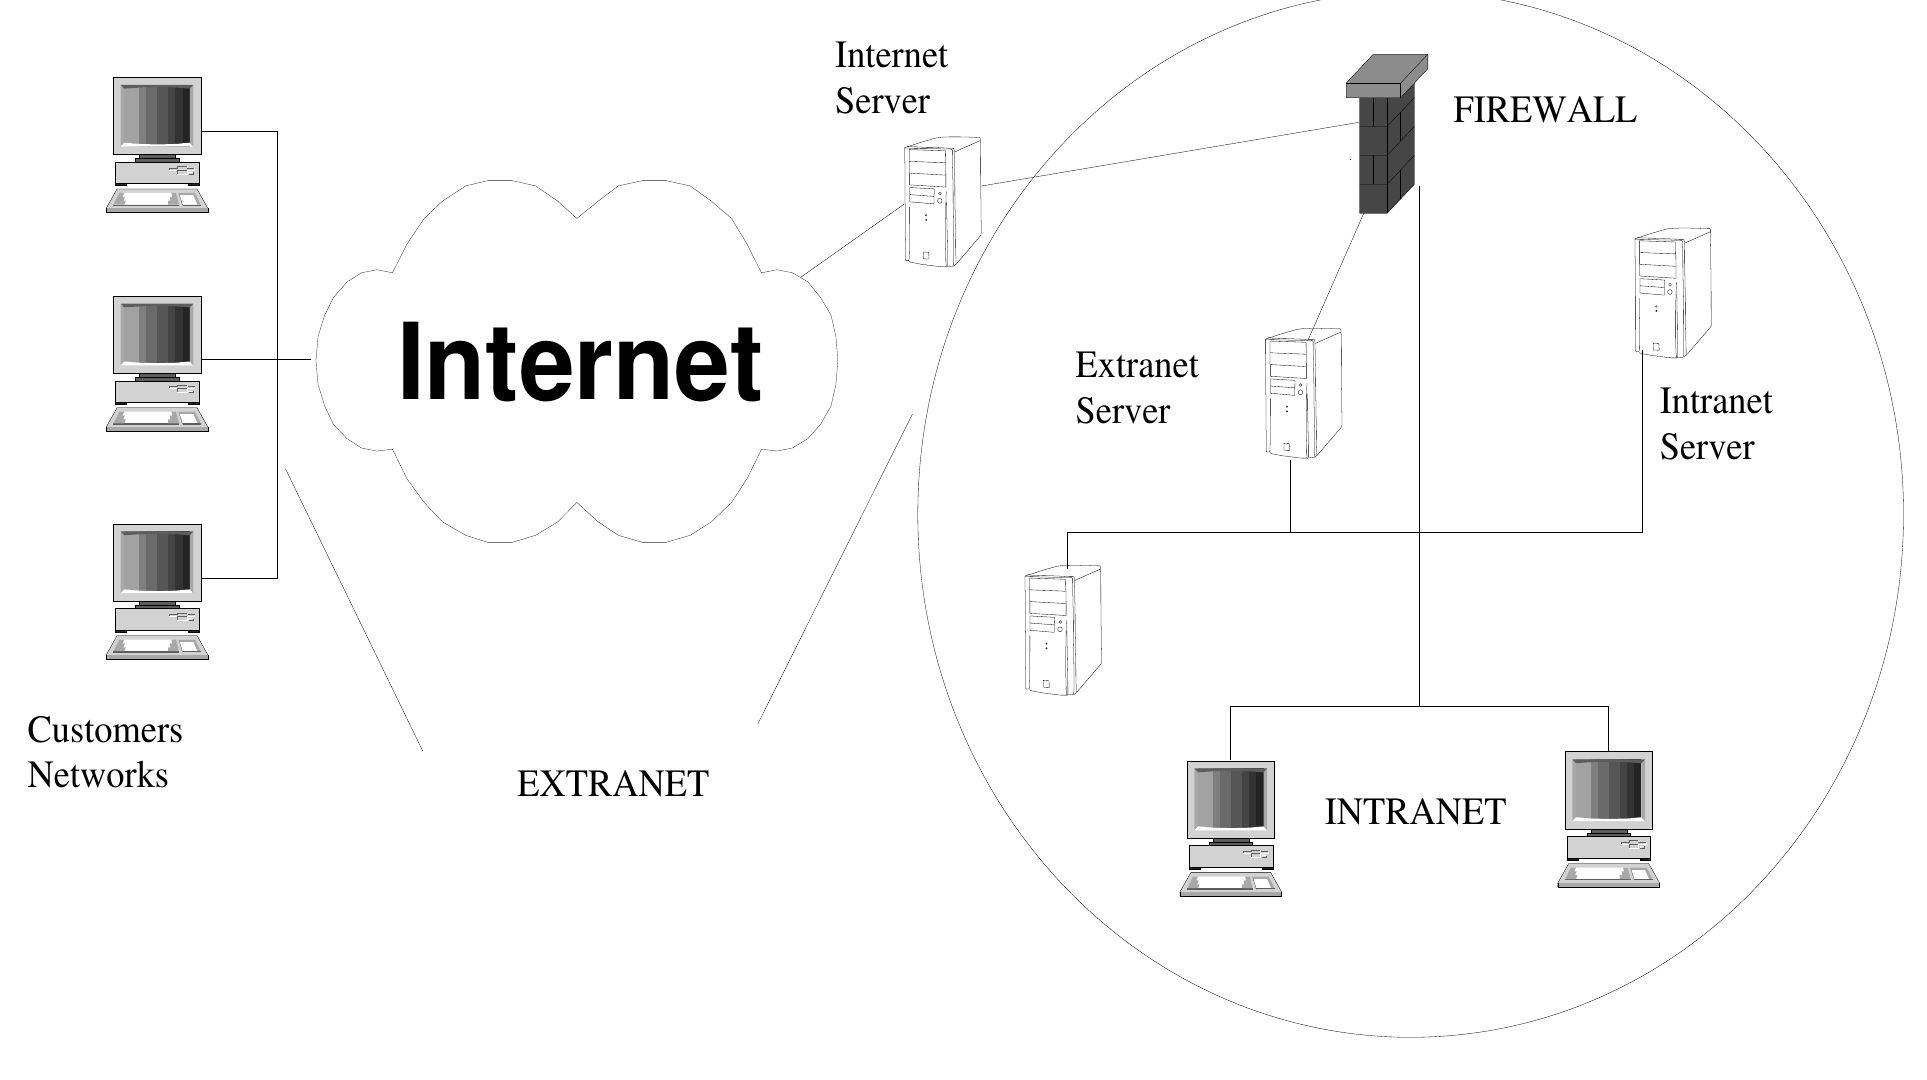
\includegraphics[width=\textwidth]{fig11_1_extranet_cloud_topology.png}

      {\scriptsize\color{accentmid}
      Figure 11.1: Similarities between a secure extranet and a private Cloud}
    \end{column}
  \end{columns}
\end{frame}

% ===================== 18. Three risk factors =====================
\begin{frame}{11.3.1 Public Cloud: Three Significant Risk Factors}
  \begin{enumerate}\small\setlength{\itemsep}{0.55em}
    \item \kw{Confidentiality and integrity of data-in-transit} to and from the
          public Cloud provider. Resources once confined to a private network
          are now exposed. HTTPS would have mitigated the integrity risk;
          users on HTTP faced data being altered without their knowledge.
    \item \kw{Proper access control} (authentication, authorization, auditing)
          for whatever resources are used at the provider. The ability to audit
          the provider's network, let alone monitor it in real time, is
          probably non-existent.
    \item \kw{Availability of the Internet-facing resources} in use or assigned
          by the provider. Reliance on network security has increased because
          more data and more personnel depend on externally hosted devices.
  \end{enumerate}
  \vspace{0.5em}

  \begin{alertblock}{Misconfiguration is still a live risk}
    \scriptsize
    A study presented to \kw{NANOG} in February 2006 found several hundred such
    misconfigurations per month. In February 2008 Pakistan Telecom announced a
    dummy route for YouTube to its partner PCCW to block the site domestically.
    \kw{YouTube was globally unavailable for two hours.}
  \end{alertblock}
\end{frame}

% ===================== 19. Trust Zones =====================
\begin{frame}{11.3.2 Trust Zones (TZ) Scheme}
  \small
  \kw{TZ} = network segmentation \textbf{+} identity and access management
  (IAM) controls, defining physical, logical or virtual \kw{boundaries} around
  network resources. Implemented with physical devices, virtual firewall and
  switching applications, or both.
  \vspace{0.7em}

  \begin{block}{Threat model: the CSP insider}
    \scriptsize
    CSP personnel with \kw{physical access} to the datacenter can breach
    controls by direct access to physical machines. The large number of
    machines complicates the task, so the attacker must first locate the
    hardware hosting the target data.
  \end{block}
  \vspace{0.5em}

  \begin{center}
  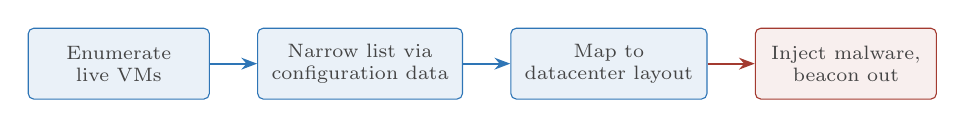
\begin{tikzpicture}[node distance=6mm]
    \node[boxy,minimum width=2.3cm,minimum height=0.9cm] (e) {Enumerate\\live VMs};
    \node[boxy,right=of e,minimum width=2.3cm,minimum height=0.9cm] (n) {Narrow list via\\configuration data};
    \node[boxy,right=of n,minimum width=2.3cm,minimum height=0.9cm] (m) {Map to\\datacenter layout};
    \node[redbox,right=of m,minimum width=2.3cm,minimum height=0.9cm] (i) {Inject malware,\\beacon out};
    \draw[flow] (e) -- (n); \draw[flow] (n) -- (m); \draw[flowred] (m) -- (i);
  \end{tikzpicture}
  \end{center}
  \vspace{0.4em}

  {\scriptsize\color{accentmid}
  Narrowing signals: security groups, open ports, IAM data, tenant naming
  conventions, relative memory / disk / CPU / IO sizing.
  \textbf{Defence:} segmented or compartmentalized datacenters, and keeping
  physical and logical maps separate, complicate the task.}
\end{frame}

% ===================== 20. PaaS application security =====================
\begin{frame}{11.4 PaaS Application Security}
  \small
  PaaS vendors fall into two categories: \kw{software vendors}
  (Bungee, Etelos, GigaSpaces, Eucalyptus) and \kw{CSPs}
  (Google App Engine, Force.com, Microsoft Azure, Intuit QuickBase).
  \vspace{0.8em}

  \begin{columns}[T,onlytextwidth]
    \begin{column}{0.49\textwidth}
      \begin{block}{Who secures what}
        \scriptsize
        PaaS CSPs secure the \kw{platform software stack}, including the
        runtime engine that runs customer applications.
        \vspace{0.4em}

        PaaS applications may use third-party applications, components or web
        services, so the \kw{third-party provider} may be responsible for
        securing those.
      \end{block}
    \end{column}
    \begin{column}{0.49\textwidth}
      \begin{block}{Practical guidance}
        \scriptsize
        Given the nascent stage of PaaS deployment, organizations evaluating
        PaaS software should perform a \kw{risk assessment} and apply the same
        software security standard as for any enterprise software.
        \vspace{0.4em}

        Customers should understand their application's dependency on all
        services and assess third-party risk.
      \end{block}
    \end{column}
  \end{columns}
  \vspace{0.8em}

  {\footnotesize\color{warmred}
  CSPs have been reluctant to share platform security information, arguing it
  would help hackers. Enterprise customers should demand \textbf{transparency}.}
\end{frame}

% ===================== 21. PaaS controls =====================
\begin{frame}{11.4 PaaS: Access Control, Hardening, SSO}
  \begin{columns}[T,onlytextwidth]
    \begin{column}{0.48\textwidth}
      \begin{block}{Access control management}
        \scriptsize
        Covers users \emph{and} privileged system administrators. Address:
        entitlement assignment, assignment based on job function,
        authentication method and strength, auditing and reporting.
      \end{block}
      \vspace{0.1em}
      \begin{block}{Hardening the host OS}
        \scriptsize
        Host OS vulnerabilities \kw{flow upward} into the VM OS. A compromise
        of the host OS gives access to \emph{all} services on \emph{all} VMs.
        \begin{itemize}\scriptsize\setlength{\itemsep}{0.05em}\setlength{\topsep}{0.2em}
          \item Strong passwords, changed often
          \item Disable unneeded services, especially networked
          \item Require full authentication
          \item Firewall the host individually
          \item Patch regularly, tested off production
        \end{itemize}
      \end{block}
    \end{column}
    \begin{column}{0.48\textwidth}
      \begin{block}{Single Sign-On (SSO)}
        \scriptsize
        One ID and password per work session, then automatic logon to all
        required applications. Passwords must never be stored or transmitted in
        the clear.
        \vspace{0.35em}

        \textbf{Advantages:} stronger passwords, easier administration, less
        time to access resources.
        \vspace{0.3em}

        \textbf{Major disadvantage:} once past the initial logon, users can
        \kw{freely roam} network resources without restriction.
        \vspace{0.35em}

        \emph{Example:} logging in to Gmail also grants YouTube, Google Drive
        and Google Photos.
      \end{block}
    \end{column}
  \end{columns}
\end{frame}

% ===================== 22. SaaS application security =====================
\begin{frame}{11.5 SaaS Application Security}
  \small
  The provider manages the \kw{entire suite} of applications, so SaaS providers
  are largely responsible for securing the applications and components they
  offer. Customers usually handle \kw{operational security}, including user and
  access management as supported by the provider.
  \vspace{0.7em}

  \begin{block}{What to request from a prospective provider}
    \small
    Design, architecture, development, black- and white-box application
    security testing, and release management.
  \end{block}
  \vspace{0.7em}

  \begin{exampleblock}{Where fine-grained control breaks down}
    \small
    Google Apps lets end users assign read and write privileges, but privilege
    management may not be fine-grained enough for an organization's access
    control standard. Embedded images in \kw{Google Docs} are not protected the
    same way the document is: once shared, the other person can still view
    those images \kw{even after sharing stops}.
  \end{exampleblock}
\end{frame}

% ===================== 23. FHE for SaaS worked example =====================
\begin{frame}{11.5.1 FHE Scheme for SaaS Security: Worked Example}
  \small
  Unlike \kw{partially} homomorphic encryption (some operations only), fully
  homomorphic encryption supports \kw{arbitrary computation} on ciphertexts. A
  program never decrypts its inputs, so an \kw{untrusted party} can run it
  without seeing inputs or internal state.
  \vspace{0.7em}

  \begin{exampleblock}{Business B and its very important data set (VIDS)}
    \begin{enumerate}\small\setlength{\itemsep}{0.25em}
      \item VIDS consists of the numbers \kw{5} and \kw{10}. To encrypt,
            Business B multiplies each element by 2, giving \kw{10} and
            \kw{20}.
      \item The encrypted set goes to the Cloud for safe storage. Months later
            the government requests the sum of VIDS elements.
      \item Business B asks the Cloud provider, which only has the encrypted
            set, to compute $10 + 20$ and returns \kw{30}.
      \item Business B decrypts the reply and gives the government the
            decrypted answer, \kw{15}.
    \end{enumerate}
  \end{exampleblock}
\end{frame}

% ===================== 24. Access control in SaaS =====================
\begin{frame}{11.5.1 Access Control in SaaS}
  \begin{columns}[T,onlytextwidth]
    \begin{column}{0.48\textwidth}
      \begin{block}{Network access control: diminishing}
        \scriptsize
        Users reach Cloud services from any Internet-connected host.
        Traditional network controls protect resources using
        \kw{host-based attributes}, which are usually inadequate, not unique
        across users, and can cause inaccurate accounting.
        \vspace{0.4em}

        In the Cloud it appears as \kw{Cloud firewall policies} at ingress and
        egress points, using standard TCP/IP parameters: source IP, source
        port, destination IP, destination port.
      \end{block}
    \end{column}
    \begin{column}{0.48\textwidth}
      \begin{block}{User access control: emphasized}
        \scriptsize
        Binds a user's \kw{identity} to Cloud resources. Supports fine granular
        access control, user accounting, compliance and data protection.
        \vspace{0.4em}

        Key controls: \kw{strong authentication}, \kw{SSO},
        \kw{privilege management}, \kw{logging and monitoring}.
        \vspace{0.4em}

        \kw{ISO/IEC 27002} defines six access control objectives covering end
        user, privileged user, network, application and information access
        control.
      \end{block}
    \end{column}
  \end{columns}
  \vspace{0.7em}
  {\footnotesize\color{accentmid}
  Customers hosting on IaaS should monitor the health of \emph{both} the hosted
  application and the virtual server instances.}
\end{frame}

% ===================== 25. Securing virtual servers =====================
\begin{frame}{11.6 Securing Virtual Servers}
  \small
  Easy \kw{self-provisioning} on IaaS creates the risk that insecure virtual
  servers get created. Secure-by-default configuration must follow or exceed
  available industry baselines.
  \vspace{0.6em}

  \begin{itemize}\scriptsize\setlength{\itemsep}{0.42em}
    \item \kw{Use a secure-by-default configuration.} Build custom VM images
          with only the capabilities and services the application stack needs.
          This limits the attack surface \emph{and} reduces patching.
    \item \kw{Track the inventory of VM images and OS versions.} Provider
          images must undergo the same verification and hardening as internal
          hosts. Best alternative: supply your own conforming image.
    \item \kw{Safeguard the private keys} for host access. Isolate decryption
          keys from the Cloud holding the data, unless they are needed there.
    \item \kw{No authentication credentials in virtualized images,} except a
          key to decrypt the filesystem key. No password-based shell access;
          passwords are mandatory for \texttt{sudo} or role-based access.
    \item \kw{Run a host firewall,} opening only the minimum ports. Turn off
          unused services such as FTP, print, network file and database
          services.
    \item \kw{Enable system auditing and event logging} to a dedicated,
          isolated log server with higher protection.
  \end{itemize}
\end{frame}

% ===================== 26. Cloud security controls =====================
\begin{frame}{11.7 Cloud Security Controls}
  \small
  Security architecture is effective only if the correct defensive
  implementations are in place. Controls safeguard weaknesses and reduce the
  effect of an attack.
  \vspace{0.5em}

  \begin{center}
  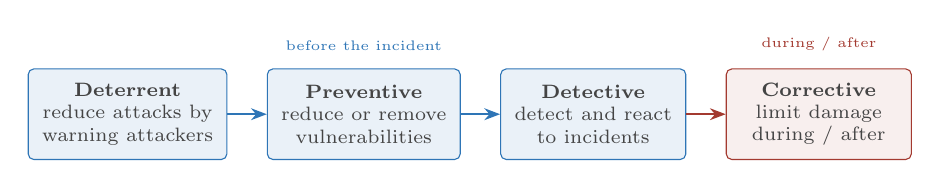
\begin{tikzpicture}[node distance=5mm]
    \node[boxy,minimum width=2.35cm,minimum height=1.15cm] (de) {\textbf{Deterrent}\\reduce attacks by\\warning attackers};
    \node[boxy,right=of de,minimum width=2.35cm,minimum height=1.15cm] (pr) {\textbf{Preventive}\\reduce or remove\\vulnerabilities};
    \node[boxy,right=of pr,minimum width=2.35cm,minimum height=1.15cm] (dt) {\textbf{Detective}\\detect and react\\to incidents};
    \node[redbox,right=of dt,minimum width=2.35cm,minimum height=1.15cm] (co) {\textbf{Corrective}\\limit damage\\during / after};
    \draw[flow] (de) -- (pr); \draw[flow] (pr) -- (dt); \draw[flowred] (dt) -- (co);
    \node[font=\tiny,color=accentmid,above=1mm of pr] {before the incident};
    \node[font=\tiny,color=warmred,above=1mm of co] {during / after};
  \end{tikzpicture}
  \end{center}
  \vspace{0.4em}

  \begin{itemize}\scriptsize\setlength{\itemsep}{0.25em}
    \item \kw{Deterrent:} like a warning sign, informs attackers of adverse
          consequences.
    \item \kw{Preventive:} strong authentication makes unauthorized access less
          likely and positive identification more likely.
    \item \kw{Detective:} system and network monitoring, intrusion detection
          and prevention; signals the preventive or corrective controls.
    \item \kw{Corrective:} restoring system backups to rebuild a compromised
          system.
  \end{itemize}
\end{frame}

% ===================== 27. Key takeaways =====================
\begin{frame}{Key Takeaways}
  \begin{itemize}\footnotesize\setlength{\itemsep}{0.45em}
    \item Cloud security is a \kw{shared responsibility}: providers secure the
          service, clients support those measures.
    \item The \kw{CIA triad} still frames the problem, but much of the stack
          now sits under third-party control.
    \item For data-in-transit the primary risk is \kw{not using a vetted
          encryption algorithm}, in any service model.
    \item \kw{ABE, FHE and SE} answer different needs: attribute-driven access,
          computation on ciphertext, secure search.
    \item A private Cloud resembles a \kw{secure extranet}; public Clouds add
          exposure, weak auditability and external availability risk.
    \item Security management works through \kw{deterrent, preventive,
          detective and corrective} controls.
  \end{itemize}
  \vspace{0.4em}

  \begin{alertblock}{From the chapter summary}
    \scriptsize
    Organizations relying solely on a vendor's built-in security expose
    themselves to unnecessary risk. Credentials and secrets proliferate across
    Cloud environments, and \kw{many are never secured}. If compromised, they
    give attackers lateral access across networks, data and applications.
  \end{alertblock}
\end{frame}

% ===================== 28. Q&A =====================
\begin{frame}[plain]
  \vfill
  \centering
  {\LARGE\bfseries\color{accent}Questions \& Discussion}

  \vspace{1.4em}
  {\small\color{accentmid}
  Chapter 11 \textbullet{} Cloud Security\par
  \vspace{0.3em}
  Manvi \& Shyam, \emph{Cloud Computing: Concepts and Technologies},
  CRC Press, 2021, pp.\ 205--227}
  \vfill
\end{frame}

\end{document}
